% =============================================================================
%  BEng Thesis — AI for Control of Soft Robot by Using ML and Inverse Kinematics
%  (Registered project title. See §1.1 Scope and terminology for the precise
%  mapping between the title keywords and the four-family IK comparative study
%  actually reported in Chapters 4-5.)
%  Format follows BEng Thesis Handbook 2025-2026.
% =============================================================================

\documentclass[12pt,a4paper,oneside]{report}
\usepackage[left=40mm,top=20mm,right=20mm,bottom=20mm]{geometry}

\usepackage{times}
\usepackage{setspace}
\usepackage{titlesec}
\usepackage{float}
\usepackage{booktabs}
\usepackage{tabularx}
\renewcommand{\tabularxcolumn}[1]{>{\RaggedRight\arraybackslash}p{#1}}
\usepackage{multirow}
\usepackage{tikz}
\usetikzlibrary{positioning, arrows.meta}
\usepackage{fancyhdr}
\usepackage{amsmath}
\usepackage{amssymb}
\DeclareMathOperator*{\argmin}{arg\,min}
\DeclareMathOperator*{\argmax}{arg\,max}
\usepackage{svg-extract}
\usepackage[justification=raggedright,singlelinecheck=false]{caption}
\usepackage{subcaption}
\usepackage{graphicx}
\usepackage{algorithmicx}
\usepackage{algpseudocode}
\usepackage{algorithm}
\usepackage{microtype}
\usepackage{ragged2e}
\usepackage{hyperref}
\usepackage{CJKutf8}
\usepackage[backend=bibtex,style=numeric,sorting=none]{biblatex}

\addbibresource{ref.bib}
\newcommand{\comment}[1]{}
\onehalfspacing

% --- Paragraph formatting (handbook: blank line between paragraphs, no indent) ---
\setlength{\parindent}{0pt}
\setlength{\parskip}{12pt plus 2pt minus 1pt}

% --- Footnotes in single spacing (handbook requirement) ---
\let\oldfootnote\footnote
\renewcommand{\footnote}[1]{\oldfootnote{\begin{singlespace}#1\end{singlespace}}}

% --- Chapter heading: 14 pt, centred, bold, block capitals (handbook §2.5) ---
%     2 double-spaced lines (~36 pt at 1.5 spacing × 12 pt) before text
\titleformat{\chapter}[display]
  {\normalfont\large\bfseries\centering}
  {\MakeUppercase{CHAPTER \thechapter}}
  {1em}
  {\MakeUppercase}
\titlespacing*{\chapter}{0pt}{50pt}{36pt}

% --- Section heading: 12 pt, left, bold, block capitals (handbook §2.6) ---
\titleformat{\section}
  {\normalfont\bfseries}
  {\thesection}
  {1em}
  {\MakeUppercase}
\titlespacing*{\section}{0pt}{3.5ex plus 1ex minus .2ex}{2.3ex plus .2ex}

% --- Subsection heading: 12 pt, left, bold, lower case (handbook §2.6) ---
\titleformat{\subsection}
  {\normalfont\bfseries}
  {\thesubsection}
  {1em}
  {}
\titlespacing*{\subsection}{0pt}{3.25ex plus 1ex minus .2ex}{1.5ex plus .2ex}

% --- Page numbers centred at foot (handbook §2.3) ---
\pagestyle{plain}
\fancyhf{}
\fancyfoot[C]{\thepage}
\renewcommand{\headrulewidth}{0pt}

\graphicspath{{fig/}}

% --- Figure caption prefix: "Fig" (handbook §6.2) ---
\renewcommand{\figurename}{Fig}

\begin{document}

% ---------- Front matter (roman page numbers) ----------
\pagenumbering{roman}

% ---------- Title page ----------
\begin{titlepage}
    \centering
    \vspace*{1cm}
    \begin{figure}[ht]
        \centering

        
\includegraphics[width=0.8\textwidth]{fig/UoD_logo.pdf}
    \end{figure}
    \vspace{1cm}
    {\huge\bfseries{Data-Driven Inverse Kinematics for Pneumatic Soft Robots: A Comparative Study of Analytical, Neural, and Jacobian-Learned Approaches}\par}
    \vspace{1.5cm}
    {\large\textbf{ }\par}
    \vspace{0.5cm}
    {\large Student ID: 2549954\par}
    \vspace{1.5cm}
    {\large Submitted for the degree of \par}
    \vspace{0.5cm}
    {\large\textbf{ }\par}
    \vspace{0.5cm}
    {\large School of Science and Engineering\par}
    \vspace{0.5cm}
    {\large University of Dundee\par}
    \vspace{0.5cm}
    {\large \par}
\end{titlepage}

\chapter{Abstract}
\thispagestyle{plain}

% Handbook §3.2: structured abstract, max 1 page, four components.

\noindent\textbf{Background:}
% TODO: pneumatic soft robots, IK challenge, limitations of existing
%       analytical and learning-based methods, motivation from Ma et al. (2022).

\noindent\textbf{Methods:}
% TODO: two datasets (DS1 I-Support, DS2 R01); four IK approaches compared
%       (PCC analytical, MLP, LSTM, Jacobian-learned); PyElastica sim-to-real;
%       trajectory tracking evaluation.

\noindent\textbf{Results:}
% TODO: headline quantitative findings (MAE/RMSE/MAPE) for best method;
%       comparison against Ma et al. (2022) MAPE<5% benchmark;
%       key ablation insight (mid-marker, temporal).

\noindent\textbf{Conclusions:}
% TODO: which IK family is recommended and under what conditions;
%       practical take-away for pneumatic soft-robot control.

\chapter{Declaration}
\thispagestyle{plain}

% TODO: standard declaration of originality. Template:
I, TODO: Author Name, student of TODO: School/Department at TODO: University, hereby declare that this thesis titled ``Data-Driven Inverse Kinematics for Pneumatic Soft Robots: A Comparative Study of Analytical, Neural, and Jacobian-Learned Approaches'' is a record of my original research work conducted under the guidance of TODO: Supervisor. All methods and ideas (unless otherwise stated) are my original creation. Any part of this thesis that is not cited has not been previously submitted for a degree at this or any other university. All sources of information and data have been properly cited.

\vspace{2cm}
\begin{flushright}
SIGNED:   \hspace{4cm} DATE: TODO
\end{flushright}

\chapter{Acknowledgments}
\thispagestyle{plain}

% TODO: acknowledge supervisor, peers, dataset authors (I-Support / Manti 2016
%   and the R01 dataset authors), any software (PyElastica) / compute support.


\tableofcontents
\listoffigures
\listoftables

\chapter{Abbreviations and Definitions}
\thispagestyle{plain}

\begin{tabular}{ll}
IK       & Inverse Kinematics \\
FK       & Forward Kinematics \\
PCC      & Piecewise Constant Curvature \\
MLP      & Multi-Layer Perceptron \\
LSTM     & Long Short-Term Memory \\
DLS      & Damped Least-Squares \\
DoF      & Degree(s) of Freedom \\
DS1      & Dataset 1 --- I-Support 20 Hz \\
DS2      & Dataset 2 --- R01 recordings \\
MAE      & Mean Absolute Error \\
RMSE     & Root Mean Squared Error \\
MAPE     & Mean Absolute Percentage Error \\
FEM      & Finite Element Method \\
SQP      & Sequential Quadratic Programming \\
% TODO: extend as new terms are introduced in the text
\end{tabular}


% ---------- Main matter (arabic page numbers) ----------
\pagenumbering{arabic}

\chapter{Introduction}
\label{chap:introduction}

\section{Scope and terminology}
\label{sec:intro_scope}

The thesis title---\emph{AI for Control of Soft Robot by Using ML and Inverse Kinematics}---frames four keywords whose scope is fixed here. \emph{AI} and \emph{ML} are used interchangeably for learning-based models trained on recorded data, instantiated as four families: feed-forward regression (§\ref{sec:bg_ik_direct}), recurrent regression (§\ref{sec:bg_ik_temporal}), Jacobian-learned iteration (§\ref{sec:bg_ik_jac}), and sim-to-real pre-training (§\ref{sec:bg_sim}). \emph{Inverse Kinematics} denotes both the analytical piecewise-constant-curvature baseline (§\ref{sec:bg_models_pcc}) and the Jacobian-learned hybrid, which inverts an ML-trained forward map iteratively at run time. \emph{Control} is taken in its open-loop position-control sense---predict the actuation command that drives the tip to a target pose---following the usage of Giorelli et al.\ \cite{giorelli2015nn}, Ma et al.\ \cite{ma2022bp}, Fang et al.\ \cite{fang2022jacobian}, and Centurelli et al.\ \cite{centurelli2022closed}. Closed-loop real-hardware control is out of scope; the evaluation closes the loop in simulation through a shared learned forward-kinematics arbiter.

\section{Motivation}
\label{sec:intro_motivation}

Soft robots deform continuously under load rather than rotating rigid joints, which makes them safer for human interaction and confined spaces but hard to control: the actuation-to-pose map is nonlinear, history-dependent, and sensitive to manufacturing asymmetries of several centimetres \cite{manti2016soft}. Pneumatic soft manipulators---silicone cylinders with internal chambers pressurised by air---are the canonical instance and the focus here.

Four inverse-kinematics method families have been proposed independently over the last decade: analytical PCC inversion, feed-forward neural regression, recurrent neural regression, and Jacobian-learned iteration on a learned forward model \cite{webster2010review, giorelli2015nn, thuruthel2019modelbased, fang2022jacobian}. Each has been evaluated on the platform its authors introduced, on different metrics, so practitioners choosing between them must assemble non-comparable experiments across papers. This thesis consolidates the four families into a single experimental programme on two complementary pneumatic datasets under identical protocols.

\section{Problem, datasets, and evaluation}
\label{sec:intro_problem}

Given a target tip position $\mathbf{x}^{\ast} \in \mathbb{R}^{3}$, predict the actuation vector $\mathbf{p} \in \mathbb{R}^{n_{p}}$ that drives the tip there. Dataset~1 is a two-module I-Support recording \cite{manti2016soft, bianchi2023learning} with six chamber pressures mapping into a three-dimensional tip (multi-valued inverse); Dataset~2 is an undocumented three-valve recording with $n_{p} = 3$ (inverse at most single-valued on the observed workspace). Evaluation uses pressure-space prediction error, closed-loop position error through the FK arbiter, and mean tracking error on four smooth reference trajectories. No physical-hardware experiments are reported.

\section{Research questions and contributions}
\label{sec:intro_rqs}

\textbf{RQ1}: Does feed-forward neural IK outperform analytical PCC, and by how much? \textbf{RQ2}: Does adding a mid-marker triad reduce pressure error on the over-actuated arm in a statistically clean paired evaluation? \textbf{RQ3}: Does a recurrent architecture improve accuracy, and under what feature conditions? \textbf{RQ4}: Does Jacobian-learned iteration produce smaller closed-loop errors, and under what actuation redundancy? \textbf{RQ5}: Does a PyElastica-pre-trained network transfer to an undocumented platform?

Four contributions address the gaps in turn: (1)~a head-to-head comparison of the four IK families on two pneumatic datasets under identical protocols; (2)~a paired mid-marker ablation quantifying partial-shape sensing on identical test frames; (3)~a sim-to-real study at four real-data budgets with an explicit negative result attributable to workspace mismatch; (4)~a three-property decision criterion (actuation redundancy, sensing coverage, target-domain overlap) synthesising the regime-specific findings into a compact method-selection framework.

\section{Thesis structure}
\label{sec:intro_structure}

Chapter~\ref{chap:background} reviews the literature along the problem, modelling, and method axes; Chapter~\ref{chap:methods} describes datasets, methods, and protocols; Chapter~\ref{chap:results} reports the experimental programme; Chapter~\ref{chap:discussion} interprets the results regime by regime and states limitations and implications; Chapter~\ref{chap:conclusion} summarises, and Chapter~\ref{chap:future_work} identifies five concrete follow-ups.

\chapter{Background and Literature Review}
\label{chap:background}

% TODO: bridging paragraph introducing the three pillars surveyed in this
%       chapter: (i) soft-robot modelling, (ii) learning-based IK, (iii)
%       simulation and sim-to-real transfer.

\section{Pneumatic soft manipulators}
\label{sec:bg_pneumatic}

The two datasets that underpin this thesis were both recorded on pneumatic soft manipulators. This section describes the design principles of that class of robot (Section~\ref{sec:bg_pneumatic_design}), the I-Support platform from which Dataset 1 was recorded (Section~\ref{sec:bg_pneumatic_isupport}), and the smaller family of three-chamber and three-valve platforms that is relevant to Dataset 2 and to the Ma et al.\ \cite{ma2022bp} benchmark (Section~\ref{sec:bg_pneumatic_others}).

\subsection{Design and actuation principles}
\label{sec:bg_pneumatic_design}

A pneumatic soft manipulator is a continuum robot whose structure deforms under fluid pressure rather than by rotating rigid links at discrete joints. The canonical design is a silicone cylinder with several sealed chambers distributed around its neutral axis; pressurising a subset of the chambers lengthens them asymmetrically relative to the others and bends the cylinder away from the active chambers. When all chambers are pressurised equally the cylinder elongates uniformly, and when only one is pressurised the cylinder bends in the plane defined by that chamber and the axis. The most common arrangement uses three chambers placed at $120^{\circ}$ around the axis, which allows bending in any direction in the plane perpendicular to the axis using only three independent pressures. Commercial and research platforms add fibre reinforcement around the chambers---typically a braided polyester or polyethylene terephthalate sheath---to constrain radial expansion and to channel pressure into axial bending or elongation.

The appeal of pneumatic actuation for soft manipulators is the combination of intrinsic mechanical compliance, safety for unstructured contact with humans, and simplicity at the drive end: pressurised air is a cheap and widely available power source, valves are small, and the actuator itself contains no internal friction surfaces. The cost is that the relationship between the applied pressure and the resulting deformation is strongly nonlinear and history-dependent. The silicone matrix exhibits viscoelastic creep on the order of seconds, so the deformation reached under a given pressure depends on the history of that pressure and not only on its current value. Manufacturing variability is also substantial: lateral displacements of $25$--$30$\,mm have been reported for otherwise identical I-Support chambers as a result of manual assembly tolerances \cite{manti2016soft}. These properties together mean that rigid-robot inverse-kinematics methods do not transfer directly to pneumatic soft arms, and they are the main reason the soft-robotics community has pursued learning-based control strategies \cite{kim2021mlsoft}.

\subsection{The I-Support platform}
\label{sec:bg_pneumatic_isupport}

The I-Support manipulator was developed by Manti et al.\ \cite{manti2016soft} at the BioRobotics Institute of Scuola Superiore Sant'Anna, originally as an assistive robot for the showering of elderly users. A single I-Support module is a silicone cylinder of $205$\,mm rest length and $60$\,mm diameter, with three McKibben-type fluidic chambers arranged at $120^{\circ}$ around the central axis and offset approximately $12$\,mm from it. The module is reinforced with a braided polyethylene terephthalate sheath that is thermally set to a bellows shape, which concentrates pressure-induced deformation into axial bending and elongation rather than radial ballooning. Each chamber can be safely pressurised up to $1.2$\,bar, at which a single-chamber actuation bends the module tip by approximately $118^{\circ}$ from its rest pose and a symmetric three-chamber actuation elongates the module by approximately $85\%$ of its rest length. These two behavioural anchors are the reference values used in the PyElastica calibration of Section~\ref{sec:sim_setup}.

Dataset 1 of this thesis was recorded on the two-module extension of the I-Support platform introduced by Bianchi et al.\ \cite{bianchi2023learning}. The two modules are stacked in series, rotated by $60^{\circ}$ relative to each other so that the six chambers together cover the full actuation circle, and mounted vertically with the end-effector pointing downwards so that gravity acts along the straight-pose axis rather than perpendicular to it. The assembled arm has a rest length of approximately $410$\,mm. These design choices together make the two-module I-Support a convenient reference platform for data-driven inverse-kinematics work on pneumatic soft robots: the actuation is pressure-only with no tendons or cables, the two-module geometry provides the six-chamber over-parameterisation that motivates multi-valued inverse methods (Section~\ref{sec:disc_interpretation}), and marker-based optical tracking of the base, mid-section, and tip provides a spatial sample of the internal configuration along the arm.

\subsection{Other pneumatic platforms relevant to this work}
\label{sec:bg_pneumatic_others}

Two further pneumatic platforms are relevant to this thesis. The first is the three-chamber single-segment arm of Ma et al.\ \cite{ma2022bp}, a purpose-built test rig developed in 2022 to evaluate a back-propagation neural network for inverse-kinematics prediction. Ma et al.'s arm uses three silicone chambers at $120^{\circ}$ around the axis without a second stage, with documented actuation units in bar and a documented straight-pose origin. Its single-segment three-chamber topology matches the geometric assumptions of the piecewise-constant-curvature model that Section~\ref{sec:bg_ik_analytical} reviews below, and the sub-$5\%$ pressure-space MAPE that Ma et al.\ reported on a $216$-sample dataset is a natural benchmark for data-driven pneumatic inverse kinematics; it is used as a scale marker for the Dataset 2 comparisons of Chapter~\ref{chap:results}.

The second is the undocumented three-valve soft arm from which Dataset 2 was recorded. The dataset was supplied by the project supervisor and is not otherwise in the public literature. From the dataset alone it is known that actuation is driven by three valves on an integer-valued command range $[0, 2500]$, that tip positions were recorded in inches and converted to millimetres, and that the observed workspace is a shallow disc of approximately $100$\,mm lateral extent and $65$\,mm axial extent (Section~\ref{sec:ds2}). The absence of documented geometry, material, and actuation calibration places Dataset 2 at the opposite extreme from Ma et al.'s platform along the documentation axis, and several of the experimental limitations discussed in Chapter~\ref{chap:discussion} trace back directly to this asymmetry.

Beyond these two specific platforms, the last decade has produced a wide variety of pneumatic soft-manipulator designs, including single-chamber bending actuators, modular multi-chamber arms, inflatable robotic trunks, and fibre-reinforced continuum manipulators; Kim et al.\ \cite{kim2021mlsoft} and Alessi et al.\ \cite{alessi2024rodreview} provide recent surveys. The present thesis draws on only two datasets, chosen because they expose complementary design properties---a two-module over-actuated pneumatic recording in Dataset 1 and an under-documented three-valve recording in Dataset 2---that together cover the actuation-redundancy regimes that the method-selection discussion of Chapter~\ref{chap:discussion} depends on.

\section{Kinematic modelling of soft robots}
\label{sec:bg_kinematics}

The inverse-kinematics methods compared in this thesis rely on an underlying model of how actuation maps to arm shape and tip position. This section reviews the three classes of kinematic model relevant to continuum soft robots: the piecewise-constant-curvature (PCC) simplification that dominates the analytical literature (Section~\ref{sec:bg_kin_pcc}), its multi-segment composition for arms with more than one module (Section~\ref{sec:bg_kin_multi}), and the more general Cosserat-rod and finite-element formulations that trade analytical tractability for physical fidelity (Section~\ref{sec:bg_kin_cosserat}).

\subsection{Piecewise constant curvature}
\label{sec:bg_kin_pcc}

The piecewise-constant-curvature (PCC) model approximates a soft manipulator's backbone as a sequence of circular arcs, each parameterised by an arc length $L$, a bending angle $\theta$ (equivalently a curvature $\kappa = \theta / L$), and an azimuth $\varphi$ that selects the plane of the bend. A single segment therefore has three configuration-space degrees of freedom, and the forward map from configuration to tip position takes a standard closed form that Webster and Jones \cite{webster2010review} derived in the most widely cited survey of continuum-robot kinematics. The appeal of PCC is its tractability: the forward kinematics is a closed-form expression in $(L, \theta, \varphi)$, the Jacobian can be written analytically, and for a single segment the inverse kinematics reduces to a system of three equations in three unknowns that can be solved in microseconds. These properties have made PCC the standard analytical baseline for pneumatic and cable-driven continuum manipulators through most of the last decade.

The tractability comes at the cost of a restrictive modelling assumption. PCC requires that the curvature is constant along every point of a segment, which in turn requires that the forces and moments acting along the segment are uniform. This assumption is approximately met on short, stiff, tendon-driven arms in which gravity and external contact are small compared with the actuation-induced bending moment. It breaks down on longer pneumatic arms subject to gravity, on arms with distributed mass or stiffness variation along the backbone, and on arms where the fluid-induced bending moment itself is not uniform. Published reviews routinely identify PCC's constant-curvature assumption as the principal source of residual error when the predicted and measured tip positions are compared on real hardware \cite{webster2010review, alessi2024rodreview}. The Dataset 2 results of Chapter~\ref{chap:results} provide one further empirical instance: the single-segment PCC baseline reaches a $22$\,mm forward residual on a workspace of only $100$\,mm because an elongation coupling that a constant-$L$ PCC cannot represent dominates the error (Section~\ref{sec:res_pcc_single}).

\subsection{Multi-segment extensions}
\label{sec:bg_kin_multi}

Multi-segment soft manipulators such as the two-module I-Support of Section~\ref{sec:bg_pneumatic_isupport} are modelled by chaining single-segment PCC transforms in series. Sokolov et al.\ \cite{sokolov2024twoseg} present an explicit two-segment derivation with a $60^{\circ}$ inter-segment rotation that corresponds to the I-Support geometry exactly, and this is the formulation adopted for the two-segment PCC baseline of Section~\ref{sec:pcc_multi}. The forward map remains closed-form under composition, but the inverse map loses its single-valued character: a two-segment arm typically has six or more actuation degrees of freedom that map into a three-dimensional tip position, and the resulting inverse is a relation rather than a function.

Two main strategies have emerged for solving the multi-segment inverse. The first is an optimisation-based search over the configuration space, constrained to physically plausible per-segment bounds; Keyvanara et al.\ \cite{keyvanara2023geometric} use sequential least-squares quadratic programming for this purpose, with a trajectory-continuity warm-start from the previous target that this thesis adopts in Section~\ref{sec:pcc_multi}. The second is a Jacobian-based iteration on the analytically tractable forward map, as developed for cable-driven continuum arms by Giorelli et al.\ \cite{giorelli2015nn}. Both approaches recover the configuration of the arm to within numerical tolerance, but they leave open how that configuration maps to the measurable actuation command; that step is straightforward when the actuation units are documented and calibrated, and it collapses under ordinary least squares when many distinct configurations share nearly the same chamber-length vector. The latter failure mode is the one observed on Dataset 1 in Section~\ref{sec:res_pcc_multi}.

\subsection{Beyond PCC: Cosserat rod and finite-element approaches}
\label{sec:bg_kin_cosserat}

When the constant-curvature assumption of PCC is violated, Cosserat-rod theory provides a more general framework that models the backbone as a continuous elastic body with cross-section orientation and position evolving along an arc-length parameter. The Cosserat rod captures nonconstant curvature under distributed loads, couples bending with elongation and torsion through the material's elastic moduli, and produces configurations that PCC cannot reach by construction. Alessi et al.\ \cite{alessi2024rodreview} review the use of rod models in continuum and soft-robot control and distinguish four main rod theories that differ in the deformation modes they represent and in how they are discretised for numerical integration. The PyElastica library of Gazzola et al.\ \cite{gazzola2018pyelastica}, which this thesis uses for the simulator of Section~\ref{sec:sim_setup}, implements the special-Cosserat-rod formulation with a position-Verlet integrator that scales linearly in the number of discretisation elements.

Higher-fidelity modelling is possible with fully three-dimensional finite-element approaches, in which the continuum is discretised into volumetric elements rather than a one-dimensional rod. Finite-element methods offer the richest physical accuracy---including contact, material nonlinearity, and stress distribution in cross-section---at substantially higher computational cost and with far more complex parameter calibration than either PCC or Cosserat-rod models. Both Cosserat-rod and finite-element models share the property that their inverse is expensive to compute directly, which is why learning-based methods that fit a fast neural surrogate to expensive simulator trajectories---the sim-to-real approach of Fang et al.\ \cite{fang2022jacobian} and of the PyElastica pipeline evaluated in Chapter~\ref{chap:results}---have become a standard route around the modelling-versus-tractability trade-off.

The practical outcome of the trade-off is that PCC remains the standard analytical baseline in soft-robot inverse-kinematics work despite its limitations: it is fast, interpretable, and accurate enough for short single-segment arms where its assumptions approximately hold. Cosserat-rod models enter when gravity, elongation, or nonconstant loading cannot be neglected, and finite-element methods are reserved for design-space studies in which simulation time is not a control-loop constraint. This thesis uses PCC as a classical reference in Section~\ref{sec:pcc_single}, the Sokolov two-segment composition in Section~\ref{sec:pcc_multi}, and a PyElastica Cosserat rod as the basis of the sim-to-real study in Section~\ref{sec:sim_setup}, covering the three regimes of the trade-off in a single experimental programme.

\section{Inverse Kinematics Methods}

\subsection{Analytical IK}
% TODO: geometric / trigonometric inversion of the PCC model; limitations
%       when the real robot deviates from the constant-curvature assumption.

\subsection{Feed-Forward Neural IK}
% TODO: MLP regressors from target pose to actuation; Giorelli et al. and
%       Ma et al. (2022) as canonical references.

\subsection{Recurrent and Temporal IK}
% TODO: LSTM / GRU for hysteresis and history-dependent deformation.

\subsection{Jacobian-Learned IK}
% TODO: Fang et al. (2022) damped least-squares scheme with a learned
%       Jacobian; pros vs. direct regression.

\section{Simulation and Sim-to-Real Transfer}

\subsection{PyElastica for Soft-Robot Simulation}
% TODO: Cosserat-rod formulation, pneumatic actuation modelling.

\subsection{Sim-to-Real Strategies}
% TODO: domain randomisation, residual learning, fine-tuning; applicability
%       to pneumatic soft arms.

\section{Evaluation Metrics and Benchmarks}

\subsection{Pose Error Metrics}
% TODO: MAE / RMSE / MAPE of tip position; percentage of workspace diameter.

\subsection{Trajectory Tracking Metrics}
% TODO: path-following error, smoothness, actuation effort.

\subsection{Published Baselines}
% TODO: headline numbers from Ma et al. (2022), Giorelli et al., Fang et al.
%       as the bar to clear.

\section{Summary and Research Gap}
% TODO: state the gap this thesis fills: a head-to-head comparison of
%       analytical, MLP, LSTM and Jacobian-learned IK on identical data,
%       plus a PyElastica sim-to-real study.

\chapter{Materials and Methods}
\label{chap:methods}

% TODO: bridging paragraph outlining the experimental programme (Exp 0--6
%       from the project plan).

\section{Datasets}

\subsection{DS1 --- I-Support (20\,Hz)}
% TODO: 2-module / 6-chamber robot, 9 optical markers, 20\,Hz random-walk
%       pressure excitation, seeds 0--3, pickle layout (N x (27 + 6)).

\subsection{DS2 --- R01 recordings}
% TODO: single-segment, 3 valves (V1..V3), (X,Y,Z) in inches; 18{,}072
%       rows, likely time-series, units conversion.

\subsection{Data Splits and Preprocessing}
% TODO: DS1: split by seed (1,2 train / 3 val / 0x3 test); base-relative
%       tip coordinates (and mid for ablation); scaler persistence.
% TODO: DS2: temporal 70/15/15 split, NEVER shuffle.

\section{Exploratory Data Analysis (Exp 0)}
% TODO: workspace shape, marker-occlusion rate, time-series verification
%       for DS2, pressure--tip correlation.

\section{Analytical Baseline: PCC Inverse Kinematics}

\subsection{Single-Segment PCC (Exp 1A, DS2)}
% TODO: equations from Ma et al. (2022) eq. 11--21 (see
%       docs/references/pcc_equations.md).

\subsection{Two-Segment PCC (Exp 1B, DS1 --- stretch goal)}
% TODO: compound PCC + SQP optimisation (see
%       docs/references/multi_segment_pcc.md).

\section{Feed-Forward Neural IK}

\subsection{MLP Architecture (Exp 2A, Tip-Only)}
% TODO: inputs (X,Y,Z), hidden layers, activation, outputs = pressures.

\subsection{Tip + Mid Ablation (Exp 2B, DS1)}
% TODO: augment inputs with mid-segment marker mean; motivation: the
%       two-segment arm is underdetermined from tip alone.

\section{Temporal IK with LSTM (Exp 3)}
% TODO: windowing strategy, sequence length, stateful vs. stateless,
%       expected benefit on hysteresis.

\section{Jacobian-Learned IK (Exp 4)}
% TODO: learned-Jacobian + damped least-squares update rule from
%       Fang et al. (2022); see docs/references/jacobian_ik_algo.md.

\section{Simulation and Sim-to-Real with PyElastica (Exp 5)}

\subsection{Simulator Setup}
% TODO: Cosserat rod params from Manti 2016; pneumatic actuation model.

\subsection{Sim-to-Real Transfer Protocol}
% TODO: pre-train on synthetic, fine-tune on real DS2; evaluation protocol.

\section{Trajectory Tracking Evaluation (Exp 6)}
% TODO: unified protocol (figure-of-eight, circle, random) applied to
%       every IK method.

\section{Training Setup and Evaluation}

\subsection{Hardware, Software and Reproducibility}
% TODO: GPU, PyTorch version, seed = 42, checkpoint metadata layout.

\subsection{Hyperparameter Selection}
% TODO: validation-set driven search; never touch the test set.

\subsection{Metrics}
% TODO: MAE / RMSE / MAPE of tip position, trajectory error, inference
%       latency.

\chapter{Results}
\label{chap:results}

% TODO: bridging paragraph: all experiments reported against identical
%       splits; headline comparison table appears in Section \ref{sec:overall}.

\section{Data Exploration Findings (Exp 0)}
% TODO: workspace plots, occlusion statistics, Dataset 2 time-series confirmation.

\section{PCC Analytical Baseline (Exp 1)}

\subsection{Single-Segment PCC on Dataset 2 (Exp 1A)}
% TODO: error distribution, failure modes.

\subsection{Two-Segment PCC on Dataset 1 (Exp 1B, if attempted)}
% TODO: note whether the stretch goal was pursued.

\section{MLP IK (Exp 2)}

\subsection{Tip-Only MLP (Exp 2A)}
% TODO: results on Dataset 1 and Dataset 2.

\subsection{Tip + Mid Ablation on Dataset 1 (Exp 2B)}
% TODO: does mid-marker input reduce error? Expected: yes, due to
%       two-segment underdetermination.

\section{Temporal LSTM IK (Exp 3)}
% TODO: comparison against MLP; hysteresis analysis.

\section{Jacobian-Learned IK (Exp 4)}
% TODO: convergence behaviour, final tip error, robustness.

\section{Sim-to-Real with PyElastica (Exp 5)}
% TODO: sim-only baseline vs. fine-tuned on real Dataset 2.

\section{Trajectory Tracking (Exp 6)}
% TODO: uniform protocol, path-following error, actuation smoothness.

\section{Overall Comparison}
\label{sec:overall}
% TODO: master table (MAE / RMSE / MAPE per method per dataset) and a
%       one-paragraph commentary on the best-performing method.

\section{Ablation Studies}
% TODO: mid-marker ablation, sequence length, damping factor for DLS,
%       simulator fine-tune ratio.

\chapter{Discussion}
\label{chap:discussion}

\section{Interpretation of results}
\label{sec:disc_interpretation}

The results of Chapter~\ref{chap:results} do not identify a single best inverse-kinematics method. Each method tested dominated some evaluation regime on some dataset, and each was beaten elsewhere. This section reads the results as a coherent story rather than as isolated experiments, argues that the regimes depend on a small number of physical properties of the system, and proposes explanations for the least obvious findings.

\paragraph{Every classical baseline failed, but for different reasons.}
The single-segment PCC of Section~\ref{sec:res_pcc_single} reached a $22$\,mm mean forward residual on the reachable subset of Dataset 2, well above the $\sim$$2$--$10$\,mm scale that would make it a competitive baseline on a workspace roughly $100$\,mm across. The diagnostic analysis attributed this to a dominant elongation signal ($r = +0.737$ between total pressurisation and tip norm) that a constant-arc-length PCC model has no degree of freedom to represent. The two-segment PCC of Section~\ref{sec:res_pcc_multi} reached geometric inverse residuals of $3 \times 10^{-3}$\,mm---essentially zero---yet its closed-loop error on Dataset 1 was $51$\,mm, roughly four times larger than the worst data-driven baseline. Here the failure is different: the geometry is fine, but the multi-valued two-segment inverse hands the linear pressure-calibration step a set of training frames whose chamber lengths collide on very different pressure commands, and ordinary least squares recovers the per-chamber mean pressure. These two failure modes are instructive because they show that a correct geometric model does not guarantee a competitive inverse: the inverse has to be well-posed both in configuration space and in actuation space, and neither dataset provides that joint well-posedness for a pure PCC pipeline.

\paragraph{Data-driven regression lets the inverse be as ill-posed as the dataset allows.}
Direct-regression networks do not need the inverse to be well-posed: when the inverse maps one tip to many pressures, the least-squares loss gently pulls the network toward the training-distribution average pressure for that tip. This is visible on Dataset 1, where the tip-only feed-forward network reached $R^{2} = 0.32$---a value that reflects a genuinely under-determined inverse, not a training failure, as confirmed by the early validation plateau at epoch $4$ (Section~\ref{sec:res_mlp_tip}). On Dataset 2, where three valves map into three tip coordinates, the inverse is essentially single-valued on the observed workspace, and the same architecture reached $R^{2} = 0.93$. This contrast is one direct argument for diagnosing the task by actuation redundancy rather than by architecture choice: the direct-regression target is the per-tip posterior mean over valid pressures, and its predictive ceiling is set by the concentration of that posterior, not by the expressive power of the network.

\paragraph{Mid-marker input lifts the posterior concentration; temporal context amplifies it.}
Adding the mid-marker coordinates to the Dataset 1 input was the largest single-factor improvement reported in this thesis ($R^{2}$ from $0.32$ to $0.44$ on the feed-forward network, from $0.28$ to $0.51$ on the recurrent network; Sections~\ref{sec:res_mlp_tipmid}, \ref{sec:res_lstm}). The information-theoretic reading is that the tip under-identifies the internal configuration of a two-segment arm, and that the mid marker supplies a partial observation of that configuration, narrowing the set of pressures consistent with the observation. Temporal context alone does \emph{not} produce this effect---the tip-only recurrent network is marginally worse than the tip-only feed-forward network on Dataset 1---yet the combination of mid-marker input and temporal context is better than either alone. The likely reason is that the recurrent network extracts the trajectory of the internal configuration rather than the trajectory of the tip, and that trajectory is a meaningful feature only once the internal configuration is itself observable. This is consistent with the hysteresis hypothesis that motivated Experiment~3 but narrows it: history helps when the features it has access to are informative enough for the history to carry physical meaning, and does not help when those features under-identify the system.

\paragraph{The Fang 2022 trade-off is a property of multi-valued inverses, not of neural architectures.}
The Jacobian-learned iteration of Section~\ref{sec:res_jacobian} was predicted to sacrifice pressure-space accuracy for position-space accuracy on a multi-valued inverse, on the grounds that direct regression averages valid solutions while a Jacobian iteration commits to one \cite{fang2022jacobian}. The measured trade-off on Dataset 2 was a $33\%$ increase in pressure MAE against a $71\%$ reduction in closed-loop position error (Table~\ref{tab:res_jacobian_pos}), and on Dataset 1 the trade-off is similar in sign but smaller in magnitude. The same reversal would be expected for any pair of methods that chooses posterior-mean versus posterior-mode behaviour on a multi-valued inverse, regardless of their implementation details. The practical consequence is that Jacobian iteration and direct regression are not ranked on a single ``quality'' scale but instead measure different objectives: a controller that places the tip in a desired position should adopt a Jacobian iteration; a system that reports pressure MAPE to a downstream consumer should adopt direct regression.

\paragraph{Sim-to-real transfer is dominated by workspace geometry, not by sample count.}
The negative sim-to-real result on Dataset 2 (Section~\ref{sec:res_sim_transfer}) is worth reading with care. Strategy~B---sim pre-training followed by real fine-tuning---matched Strategy~A at every real-data budget tested, including the $10\%$ budget at which one would most expect a prior to help. Strategy~C, which used only synthetic data, failed with $R^{2} = -1.71$ on Dataset 2. The synthetic workspace produced by the calibrated rod of Section~\ref{sec:res_sim_cal} was five times the linear extent of Dataset 2 on every axis and centred in a different region of tip space, so the pre-training distribution had almost no overlap with the test distribution. Under these conditions the pre-training is not a prior toward the right answer but a prior toward an irrelevant answer, and fine-tuning on a small fraction of real data discards most of the pre-trained weights. The more general reading is that a Manti-inspired rod is not a drop-in prior for an undocumented robot: the value of any such prior is bounded above by the overlap between its synthetic workspace and the real operating region, and the $720$-sample count that limited the present simulation is not the reason this ceiling was hit.

\paragraph{A compact decision criterion.}
Across the six methods and two datasets tested here, the right inverse-kinematics method for a new pneumatic soft-robot arm is determined less by the method itself than by three properties of the arm and its intended use. First, actuation redundancy: if there are more actuation degrees of freedom than tip degrees of freedom, a Jacobian-based iteration can be expected to drive closed-loop error to the tolerance floor, as observed on the six-chamber Dataset 1 arm. Second, sensing coverage: if the tip under-identifies the internal configuration, additional observations---mid markers, full-shape sensing, or any other partial observation of the internal state---lift the predictive ceiling more than any network-architecture change, as observed on Dataset 1 with the mid-marker ablation. Third, target-domain overlap: a simulator prior is useful only when its synthetic workspace covers the intended operating region of the real arm; otherwise the most data-efficient route is still to train on real data alone, as observed on Dataset 2. These three properties together recover most of the regime-specific findings of Chapter~\ref{chap:results} and give a compact decision criterion that does not privilege any single method.

\section{Comparison with Published Baselines}
% TODO: explicit comparison with Ma et al. (2022) (MAPE~<5\%) and other
%       benchmarks from docs/references/giorelli_nn_vs_jacobian.md.

\section{The Role of Mid-Segment Information (Dataset 1)}
% TODO: discuss why tip-only IK is underdetermined for two-segment arms
%       and what this implies for sensing requirements.

\section{Temporal Modelling and Hysteresis}
% TODO: when does LSTM help, when not; limits of the tested sequence
%       lengths.

\section{Jacobian vs. Direct Regression}
% TODO: generalisation, sample efficiency, robustness to out-of-distribution
%       targets.

\section{Sim-to-Real Observations}
% TODO: what transfers, what does not; the reality gap for pneumatic
%       actuation dynamics.

\section{Limitations}

\subsection{No Physical Robot}
% TODO: all evaluation is on pre-recorded datasets; no closed-loop testing.

\subsection{Dataset Coverage}
% TODO: two datasets, two geometries; broader generalisation unverified.

\subsection{Simulator Fidelity}
% TODO: PyElastica limitations (no air dynamics, simplified hysteresis).

\subsection{Metric Choice}
% TODO: tip-only error ignores shape; implications for downstream use.

\section{Implications}
% TODO: practical take-aways for practitioners choosing an IK strategy
%       for a new pneumatic soft arm.

\chapter{Conclusion}
\label{chap:conclusion}

This thesis evaluated four families of inverse-kinematics method on two pneumatic soft-robot datasets---a two-module six-chamber I-Support recording and an undocumented three-valve recording---under identical training and evaluation protocols. The methods compared were analytical piecewise-constant-curvature inverse kinematics in single- and two-segment formulations, feed-forward neural inverse kinematics in tip-only and tip-plus-mid input configurations, recurrent neural inverse kinematics in the same two input configurations, and Jacobian-learned iterative inverse kinematics. A sim-to-real transfer study using a calibrated PyElastica rod at four real-data budgets, and a four-trajectory tracking evaluation applied uniformly to every method, completed the experimental programme.

The headline quantitative findings are as follows. The analytical piecewise-constant-curvature baseline is not competitive with even a small feed-forward network on either dataset, for two distinct reasons: a constant-arc-length structural ceiling produced a $22$\,mm forward residual on Dataset 2, and a multi-valued-inverse calibration collapse produced a $51$\,mm closed-loop error on Dataset 1 despite a near-zero geometric residual. Adding the mid-marker coordinates to the Dataset 1 input reduced pressure MAE by $15\%$ on the feed-forward network and raised the coefficient of determination from $0.32$ to $0.44$; combining the mid-marker input with a recurrent architecture lifted the coefficient of determination further to $0.51$, the best Dataset 1 result reported in this thesis. The warm-started Jacobian-learned iteration reached $0.71$\,mm mean closed-loop position error on the per-sample Dataset 1 test sub-sample and $0.77$\,mm on the reference trajectories, hitting the DLS solver's $1$\,mm tolerance on every Dataset 1 trajectory target; on the under-actuated Dataset 2 the same iteration diverged on the helical spiral and lost the advantage, and a sim-to-real-fine-tuned feed-forward network was the best Dataset 2 tracker at $6.20$\,mm. The sim-to-real pre-training produced no measurable improvement in pressure-space accuracy on Dataset 2 at any real-data budget, a negative result attributable to a five-fold workspace mismatch between the I-Support-inspired simulator and the target robot rather than to the real-data sample count.

Against the published literature, the Dataset 1 sub-millimetre Jacobian result matches the order of magnitude reported by Fang et al.\ \cite{fang2022jacobian} for learned-Jacobian inverse kinematics on a different pneumatic platform, and the feed-forward-over-analytical improvement on Dataset 2 matches the factor-of-two pattern reported by Giorelli et al.\ \cite{giorelli2015nn} on a cable-driven soft arm. The sub-$5\%$ pressure-space MAPE benchmark of Ma et al.\ \cite{ma2022bp} was not reached on Dataset 2; most of the gap is attributable to the undocumented actuation units and zero-frame of Dataset 2 rather than to any limitation of the methods themselves.

Taken together, these findings support a single synthesis. The right inverse-kinematics method for a new pneumatic soft-robot arm depends on three properties of the arm and its intended use---actuation redundancy, sensing coverage, and target-domain overlap---and no single method tested here dominated every combination of those properties. Where actuation redundancy is available and partial-shape sensing is present, as on the two-module I-Support recording, the warm-started Jacobian-learned iteration drives closed-loop error to the solver tolerance; where actuation matches the output dimension and no documented digital twin is available, as on the three-valve recording, a feed-forward network with or without sim-to-real pre-training remains the best option. The three-property criterion organises the regime-specific results of the experimental programme into a compact method-selection framework for practitioners who have to choose an inverse-kinematics method for a new pneumatic soft-robot arm.

These findings operationalise the title of this thesis. \emph{AI for Control of Soft Robot by Using ML and Inverse Kinematics} has been instantiated here, per the scope fixed in Section~\ref{sec:intro_scope}, as (i) \emph{AI} and \emph{ML} in the form of four learning-based families---feed-forward regression, recurrent regression, Jacobian-learned iteration, and sim-to-real fine-tuning; (ii) \emph{Inverse Kinematics} in the form of both the analytical piecewise-constant-curvature baseline and the Jacobian-learned hybrid, which inverts an ML-trained forward map iteratively at run time and therefore combines \emph{ML} and \emph{IK} in a single architecture; and (iii) \emph{Control of Soft Robot} in its open-loop position-control sense, evaluated on the four-trajectory tracking protocol through a shared learned forward-kinematics arbiter. Within this scope, the three-property decision criterion above gives the practical shape of an answer to the title question: which AI instantiation best controls a soft robot depends on the platform's actuation redundancy, its sensing coverage, and the overlap between any simulator prior and its real operating workspace---and the experimental evidence of Chapter~\ref{chap:results} quantifies that dependence on two complementary pneumatic datasets. Closed-loop real-hardware validation of the controlled arm remains the natural next step, as discussed in Chapter~\ref{chap:future_work}.

\chapter{Future Work}
\label{chap:future_work}

% TODO: candidate directions, e.g.
%   1) Closed-loop validation on a physical pneumatic arm.
%   2) Full-shape IK (predicting mid markers) beyond the tip.
%   3) Higher-fidelity FEM simulation (SOFA) and broader sim-to-real tests.
%   4) Online hysteresis compensation with recurrent Jacobian-learned IK.
%   5) Multi-task / multi-robot transfer learning across platforms.


% ---------- References ----------
\sloppy
\printbibliography[title={References}]

% ---------- Appendices (handbook: each numbered with a suitable title) ----------
\appendix
\chapter{Supervision Records}
\label{app:supervision}

% Handbook §4.2: 8 signed supervision forms must be scanned and attached
%                as Appendix A.

% TODO: include scanned signed supervision forms (8 meetings).
%       Example:
%       \includegraphics[width=\textwidth]{fig/supervision_form_1.pdf}
%       \newpage
%       \includegraphics[width=\textwidth]{fig/supervision_form_2.pdf}
%       ... (repeat for all 8 forms)

\chapter{Risk Assessment}
\label{app:risk}

% Handbook §4.3: a copy of the Risk Assessment form must be included.

% TODO: include the completed Risk Assessment form. If the project is
%       entirely software-based with publicly available datasets, state so
%       and include the signed form confirming no significant risks.
%
%       \includegraphics[width=\textwidth]{fig/risk_assessment_form.pdf}

\input{chapters/appendix_C_derivations}
\chapter{Extended Results}
\label{app:extended}

This appendix collects the hyperparameter configurations, supplementary figures, and environment details that scale and reproduce the results of Chapter~\ref{chap:results}. The material here is referenced from the main text where it supports a specific claim; none of the numbers reported in Chapters~\ref{chap:results}--\ref{chap:conclusion} depend on reading this appendix.

\section{Hyperparameter configurations}
\label{app:hyperparameters}

Table~\ref{tab:app_hyperparams_networks} lists the final hyperparameters for every trained inverse-kinematics or forward-kinematics network reported in Chapter~\ref{chap:results}. Architecture widths, optimiser, learning rate, batch size, epoch cap, early-stopping patience, random seed, and the best-epoch indices returned by the early-stopping monitor are shown. All values are those fixed after the preliminary sweeps described in Section~\ref{sec:hyperparam}; they are identical across both datasets unless the $n_{p}$-dependent output width is indicated.

\begin{table}[!htbp]
  \centering
  \footnotesize
  \setlength{\tabcolsep}{4pt}
  \caption{Final hyperparameter configurations for every trained network, matched to the registered YAML configurations in \texttt{configs/*.yaml}. Output width equals $n_{p}$ for inverse-kinematics networks and $3$ for forward-kinematics networks. MLP architectures are reported as input--hidden$_{1}$--hidden$_{2}$--hidden$_{3}$--hidden$_{4}$--output (four hidden layers throughout); LSTM architectures are reported as (window $W$, hidden units, layers). All networks use ReLU (MLP) or default PyTorch tanh/sigmoid (LSTM) activations, the Adam optimiser, and seed $42$. Input features are $(x,y,z)$ for tip-only IK networks, $(x,y,z,x_{m},y_{m},z_{m})$ for tip-plus-mid IK networks, and the pressure/valve command vector for FK arbiters.}
  \label{tab:app_hyperparams_networks}
  \begin{tabularx}{\linewidth}{@{}l l X l l l l@{}}
    \toprule
    Role & Dataset & Architecture & Lr & Batch & Cap / pat. & Best ep. \\
    \midrule
    IK MLP tip-only         & Dataset 1 & 3--128--256--256--128--6  & $10^{-3}$ & 64 & 500 / 30 & 4   \\
    IK MLP tip-plus-mid     & Dataset 1 & 6--128--256--256--128--6  & $10^{-3}$ & 64 & 500 / 30 & 21  \\
    IK MLP tip-only         & Dataset 2 & 3--64--128--128--64--3    & $10^{-3}$ & 64 & 500 / 30 & 44  \\
    IK LSTM tip-only        & Dataset 1 & ($W{=}10$, $128$, $2$)    & $10^{-3}$ & 64 & 300 / 20 & 38  \\
    IK LSTM tip-plus-mid    & Dataset 1 & ($W{=}10$, $128$, $2$)    & $10^{-3}$ & 64 & 300 / 20 & 45  \\
    IK LSTM tip-only        & Dataset 2 & ($W{=}10$, $128$, $2$)    & $10^{-3}$ & 64 & 300 / 20 & 114 \\
    FK arbiter              & Dataset 1 & 6--128--256--256--128--3  & $10^{-3}$ & 64 & 500 / 30 & 82  \\
    FK arbiter              & Dataset 2 & 3--64--128--128--64--3    & $10^{-3}$ & 64 & 500 / 30 & 156 \\
    Sim2Real Strategy A     & Dataset 2 & 3--64--128--128--64--3    & $10^{-3}$ & 64 & 500 / 30 & 137 \\
    Sim2Real B (pre-train)  & synthetic & 3--64--128--128--64--3    & $10^{-3}$ & 64 & 100 / --- & --- \\
    Sim2Real B (fine-tune)  & Dataset 2 & 3--64--128--128--64--3    & $10^{-4}$ & 64 & 500 / 30 & 71  \\
    Sim2Real Strategy C     & synthetic & 3--64--128--128--64--3    & $10^{-3}$ & 64 & 500 / 30 & 198 \\
    \bottomrule
  \end{tabularx}

  \vspace{0.5em}
  \noindent\emph{Note.} Strategy~B's pre-training phase runs for a fixed cap of $100$ epochs with no early-stopping monitor, so no best-epoch index is reported for that phase; both phases of Strategy~B share the same network architecture and scalers, which are fitted on the real subset so the synthetic pre-training data is transformed into the target-domain standardisation (Section~\ref{sec:sim_transfer}). The Dataset~2 MLP best-epoch of $44$ matches the training-curve dotted marker of Figure~\ref{fig:app_training_curves}; the FK arbiter and Dataset~2 LSTM values are read from their respective training runs on the same configuration.
\end{table}

Table~\ref{tab:app_hyperparams_solvers} collects the hyperparameters of the non-learned components: the SLSQP two-segment PCC inverse of Section~\ref{sec:pcc_multi} and the damped-least-squares Jacobian iteration of Section~\ref{sec:jacobian}. These values were fixed in advance from the referenced literature and are reported here for completeness.

\begin{table}[!htbp]
  \centering
  \small
  \caption{Hyperparameters of the optimisation-based and iterative solvers.}
  \label{tab:app_hyperparams_solvers}
  \begin{tabularx}{\linewidth}{@{}l l X@{}}
    \toprule
    Component & Parameter & Value \\
    \midrule
    \multirow{4}{*}{Two-segment PCC SLSQP} & Bounds $\theta_{s}$            & $[0,\, 2.5]$\,rad per segment \\
                                            & Bounds $\varphi_{s}$           & $[-\pi,\, \pi]$\,rad per segment \\
                                            & Bounds $\Delta L_{s}$          & $[-50,\, +50]$\,mm per segment \\
                                            & Termination tolerance          & $10^{-8}$ on objective gradient \\
    \midrule
    \multirow{6}{*}{Jacobian DLS iteration} & Damping $\lambda$              & $0.05$ \\
                                            & Step scale $\alpha$            & $0.5$ \\
                                            & Position tolerance             & $1$\,mm \\
                                            & Max iterations                 & $50$ \\
                                            & Jacobian mode                  & PyTorch autograd on FK net \\
                                            & Initialisation                 & cold (mid-range) \textit{or} warm (MLP prediction) \\
    \bottomrule
  \end{tabularx}
\end{table}

\section{Exploratory data analysis: protocol}
\label{app:eda_protocol}

Each dataset was examined before model training to verify raw-data format, validate the preprocessing assumptions of Section~\ref{sec:splits}, and (for Dataset~1) estimate the physical noise floor.

\paragraph{Dataset~1 checks.}
(i) Per-recording spatial standard deviation of the base-marker mean position, as a base-stationarity check within each recording. (ii) Overlaid four-seed base-relative tip point clouds, as a check for rotational drift between recording sessions. (iii) Seed-0 repeatability from the three repeated trials: each tip sample in one trial was paired with its nearest neighbour in the other two trials in the six-dimensional pressure-command space, and the standard deviation of the three paired tip positions was recorded per frame. Nearest-neighbour matching was preferred over index alignment because the seed-0 command sequences differed slightly across trials; see Appendix~\ref{app:eda_detail}.

\paragraph{Dataset~2 checks.}
(i) Missing-value and duplicate-row counts. (ii) Per-column histograms for truncation, clipping, or quantisation artefacts. (iii) A shuffled-vs-ordered step-size ratio to test whether consecutive rows carry any temporal dependency: the mean Euclidean step between consecutive rows was compared against the analogous statistic under row permutation, in both tip-position space and valve-command space. (iv) Pearson correlations between each valve command and each tip coordinate as a non-degeneracy sanity check on the actuation--pose map.

\section{Exploratory data analysis: findings in detail}
\label{app:eda_detail}

\paragraph{Dataset~1 occlusion.}
All six recordings contain exactly $4{,}000$ raw frames ($24{,}000$ total). Marker drop-outs lost $64$ frames in aggregate ($0.27\%$), distributed unevenly across recordings (Table~\ref{tab:app_eda_ds1_occlusion}). The mid and tip triad occlusion masks were identical per recording, so the same $23{,}936$ frames remain usable for both the tip-only and the tip-plus-mid variants.

\begin{table}[!htbp]
  \centering
  \small
  \caption[Per-recording occlusion counts for Dataset~1.]{Per-recording occlusion counts for Dataset~1. Each recording contains $4{,}000$ raw frames; usable frames are those in which every marker in the mid and tip triads was visible.}
  \label{tab:app_eda_ds1_occlusion}
  \begin{tabularx}{\linewidth}{@{}l l X X X@{}}
    \toprule
    Seed & Trial & Raw frames & Usable frames & Occlusion \\
    \midrule
    1 & 1 & $4{,}000$ & $3{,}981$ & $0.48\%$ \\
    2 & 1 & $4{,}000$ & $4{,}000$ & $0.00\%$ \\
    3 & 1 & $4{,}000$ & $3{,}999$ & $0.03\%$ \\
    0 & 1 & $4{,}000$ & $3{,}990$ & $0.25\%$ \\
    0 & 2 & $4{,}000$ & $4{,}000$ & $0.00\%$ \\
    0 & 3 & $4{,}000$ & $3{,}966$ & $0.85\%$ \\
    \bottomrule
  \end{tabularx}
\end{table}

\paragraph{Dataset~1 base stationarity.}
Five of six recordings showed apparent base motion of up to $\sim$$32$\,mm in the per-frame base-mean spatial standard deviation; inspection of the raw marker stream showed this was an NaN-aware-mean artefact (when one or two of the three base markers were momentarily occluded, the mean collapsed onto the remaining marker's cluster-centroid offset). Once occluded frames were removed, the standard deviation fell below optical marker resolution, so the base is treated as fixed within every recording and the translation-only preprocessing of Section~\ref{sec:splits} is justified.

\paragraph{Dataset~1 tip and mid magnitudes.}
Mean base-relative tip magnitude $\approx 375$\,mm (max $\approx 405$\,mm, consistent with the $\sim$$410$\,mm assembled length); mean mid magnitude $\approx 198$\,mm, consistent with the mid-section sitting near the arm midpoint. Both fall within the $500$\,mm sanity threshold of the loader.

\paragraph{Dataset~1 seed-0 repeatability distribution.}
The paired per-frame tip standard deviation across the three seed-0 trials has mean $2.29$\,mm, median $1.88$\,mm, and $95$th percentile $4.14$\,mm, with a long tail to $60.3$\,mm driven by isolated frames near occlusion gaps (Fig~\ref{fig:app_ds1_repeatability}). The $\sim$$2.3$\,mm mean is cited as the Dataset~1 physical noise floor in Section~\ref{sec:eda_findings} and subsequent chapters.

\begin{figure}[!htbp]
  \centering
  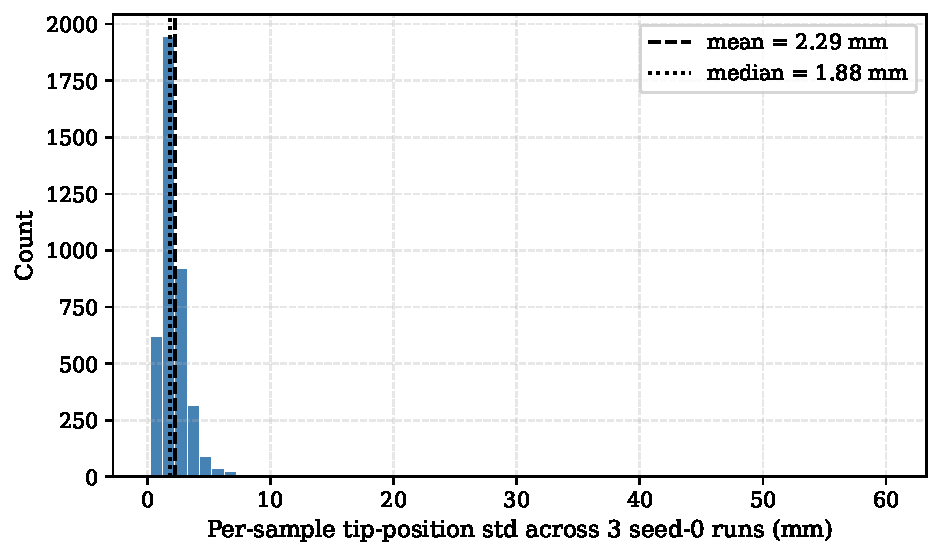
\includegraphics[width=0.75\linewidth]{fig/ds1_seed0_repeatability.pdf}
  \caption[Seed-0 repeatability distribution for Dataset~1.]{Per-sample tip-position standard deviation across the three repetitions of the Dataset~1 seed-0 recording, with frames paired by nearest neighbour in the six-dimensional pressure-command space.}
  \label{fig:app_ds1_repeatability}
\end{figure}

\paragraph{Dataset~1 seed-0 command non-identity.}
Contrary to the expectation set by a shared RNG seed, the three seed-0 pressure-command sequences were not bit-identical: mean per-frame Euclidean distance between repetition 1 and 2 was $13.2$ raw units, between 1 and 3 was $45.2$ raw units (range $[0, 100]$). Index-aligned pairing would therefore compare slightly different commands, which is why the nearest-neighbour matching above was adopted.

\paragraph{Dataset~2 integrity.}
$18{,}072$ rows, no missing values, no duplicate rows. Valve commands integer-valued in $[0, 2500]$; every row inside this band. After inch-to-millimetre conversion the tip coordinates span $[-47.9, 53.8]$\,mm ($X$), $[-47.7, 56.1]$\,mm ($Y$), $[-27.5, 36.9]$\,mm ($Z$).

\paragraph{Dataset~2 temporal structure (absent).}
Mean Euclidean consecutive-row step in tip-position space $32.49$\,mm, versus $33.84$\,mm under row permutation (ratio $0.96$). The same statistic in three-dimensional valve-command space gives ratio $1.003$. Both ratios are indistinguishable from unity, so the rows of Dataset~2 behave as IID samples rather than as a trajectory. The default $70/15/15$ order-preserving split of Section~\ref{sec:splits} was retained as a precaution against subtle residual structure.

\paragraph{Dataset~2 actuation--pose correlation.}
Every valve--coordinate Pearson coefficient has magnitude above $0.09$ (Fig~\ref{fig:app_ds2_correlation}); the strongest entries are consistent with three chambers at $120^{\circ}$ (valve~1: $-Y, +Z$; valve~2: $+X$; valve~3: $-X$). The actuation--pose map is non-degenerate.

\begin{figure}[!htbp]
  \centering
  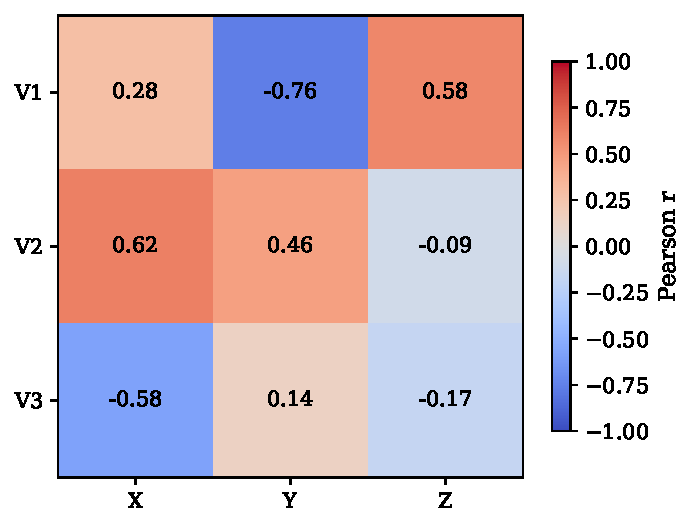
\includegraphics[width=0.6\linewidth]{fig/ds2_correlation.pdf}
  \caption[Actuation--pose correlation matrix for Dataset~2.]{Pearson correlation between each valve command and each tip coordinate across the $18{,}072$ rows of Dataset~2. The strongest per-row entries are consistent with a three-chamber radial actuator at $120^{\circ}$.}
  \label{fig:app_ds2_correlation}
\end{figure}

\section{Supplementary figures}
\label{app:extended_figures}

Figure~\ref{fig:app_training_curves} shows the training and validation loss curves for the feed-forward networks of Section~\ref{sec:res_mlp_tip} on both datasets. The Dataset~1 curve flattens around epoch $4$ and the validation loss starts to increase thereafter, so early stopping selects the fourth-epoch checkpoint and confirms the data-limited plateau discussed in Section~\ref{sec:disc_jacobian_vs_mlp}. The Dataset~2 curve continues to descend for several tens of epochs before levelling off, with the validation-loss minimum at epoch~$44$; this is consistent with the single-valued inverse being learnable from the available sample count.

\begin{figure}[!htbp]
  \centering
  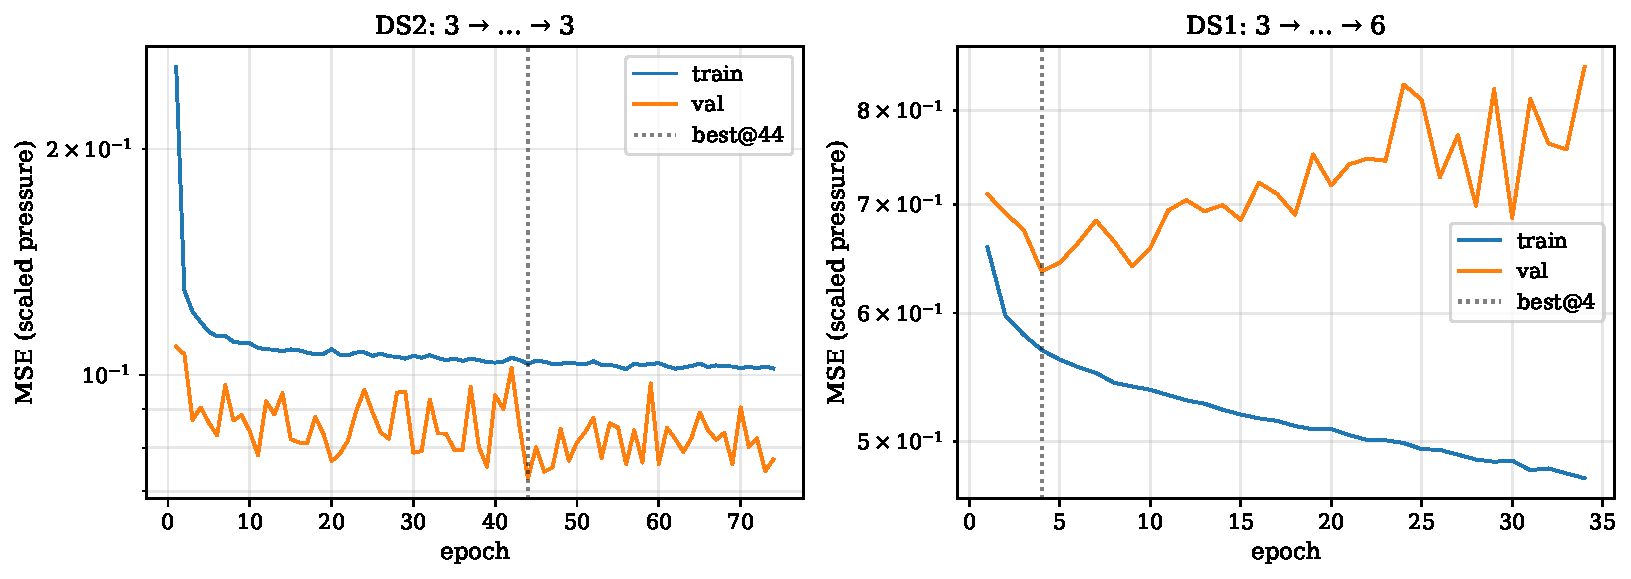
\includegraphics[width=0.92\linewidth]{fig/mlp_training_curves.pdf}
  \caption[Training and validation loss of the tip-only MLPs.]{Training and validation loss as a function of epoch for the tip-only MLP on Dataset~2 (left) and Dataset~1 (right). The vertical axis is mean squared error on the $z$-score-standardised pressure targets (not raw-unit MAE), the loss function actually optimised during training; raw-unit MAE is reported in the main results tables. Vertical dotted lines mark the early-stopping best-epoch indices ($44$ for Dataset~2, $4$ for Dataset~1), which are the indices recorded in Table~\ref{tab:app_hyperparams_networks}.}
  \label{fig:app_training_curves}
\end{figure}

Figure~\ref{fig:app_mlp_sweep} presents the hyperparameter sweep heatmap referenced in Section~\ref{sec:hyperparam}. Each cell reports the validation pressure MAE at the corresponding $(\text{hidden width}, \text{learning rate})$ combination on Dataset~2; the $128$-unit, $10^{-3}$ configuration chosen for all subsequent experiments is inside the region of flat near-optimal performance.

\begin{figure}[!htbp]
  \centering
  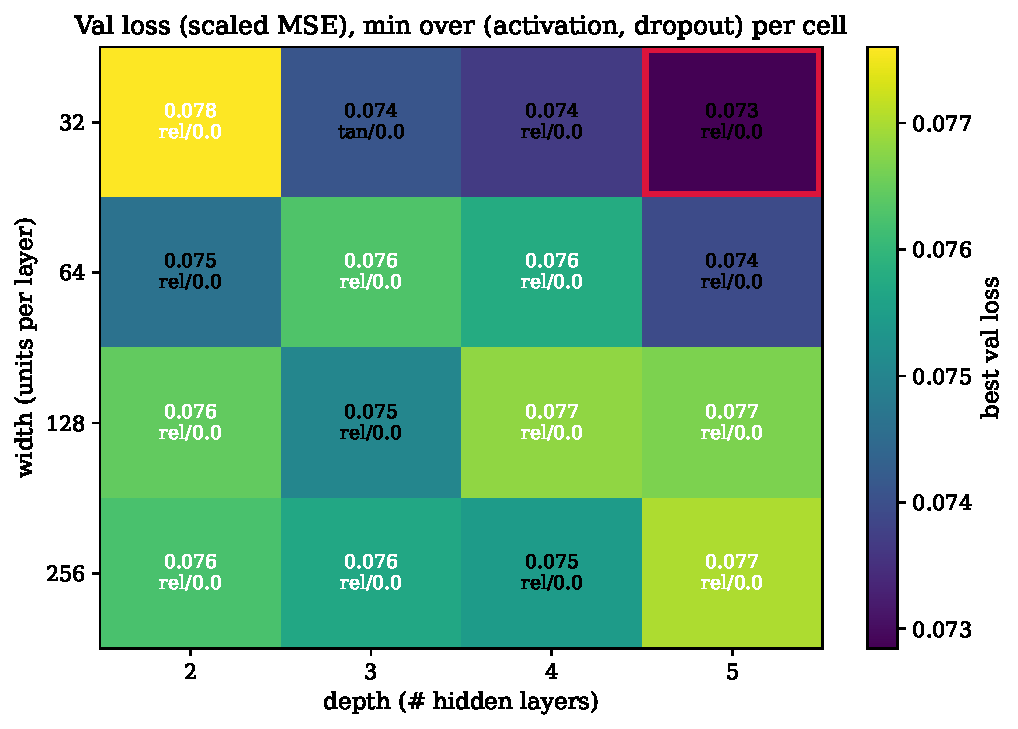
\includegraphics[width=0.78\linewidth]{fig/mlp_sweep_heatmap.pdf}
  \caption[Validation pressure MAE across the MLP hyperparameter sweep on Dataset~2.]{Validation pressure MAE across the MLP hyperparameter sweep on Dataset~2. Darker cells denote lower error. The configuration selected for all reported MLP experiments is marked with a white frame.}
  \label{fig:app_mlp_sweep}
\end{figure}

Figure~\ref{fig:app_jacobian_time} shows the per-target inference-time distribution of the warm-started Jacobian-learned iteration on both datasets, alongside the constant-cost feed-forward MLP baseline, as referenced in Section~\ref{sec:res_jacobian}. The Jacobian histogram is tightly peaked around $46$\,ms on both datasets, two to three orders of magnitude slower than the $\sim\!0.05$\,ms per-target MLP evaluation. The logarithmic horizontal axis makes the size of the latency gap visible at a glance.

\begin{figure}[!htbp]
  \centering
  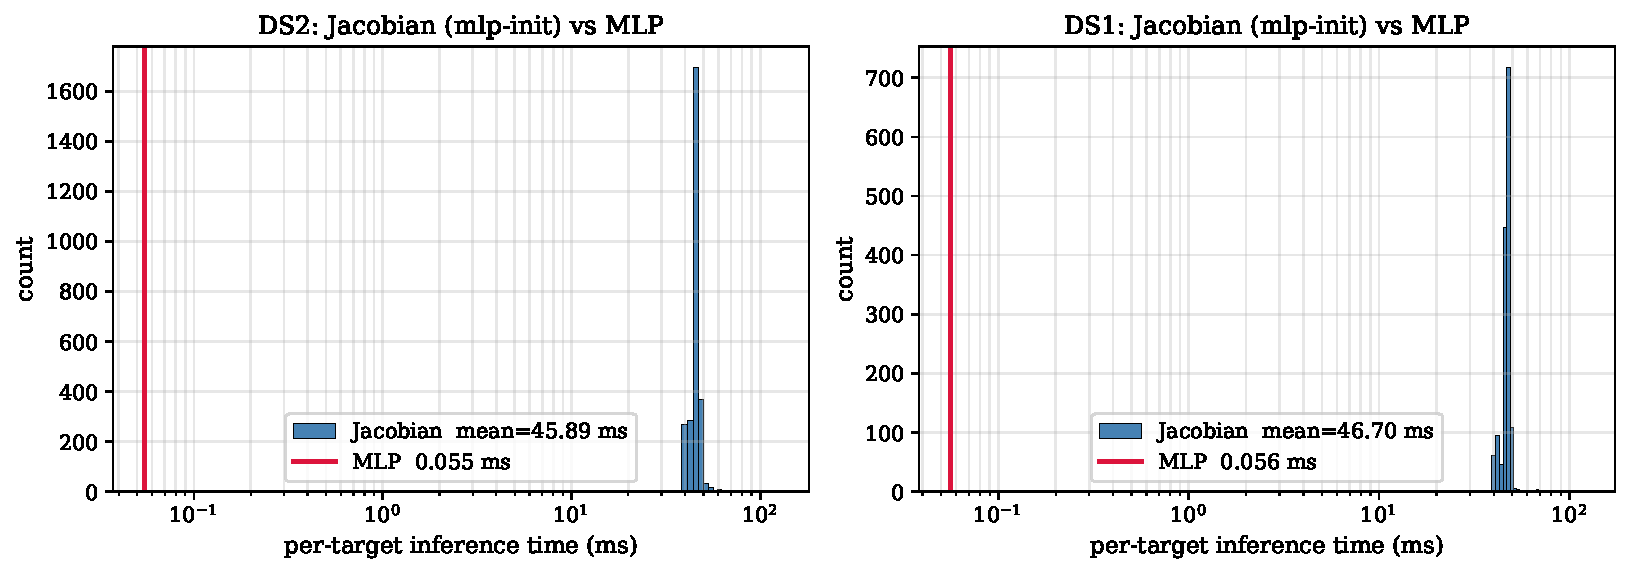
\includegraphics[width=0.95\linewidth]{fig/jacobian_inference_time.pdf}
  \caption[Per-target inference-time distributions: Jacobian-IK vs MLP.]{Distribution of per-target wall-clock inference time for the warm-started (MLP-initialised) Jacobian-learned iteration (blue histogram) and the feed-forward MLP baseline (red vertical line) on Dataset~2 (left) and Dataset~1 (right). The horizontal axis is logarithmic (milliseconds). Jacobian means are $45.89$\,ms on Dataset~2 and $46.70$\,ms on Dataset~1, against $0.055$\,ms and $0.056$\,ms for the MLP respectively; the Jacobian iteration is therefore roughly $830\times$ slower than the direct regressor on both platforms.}
  \label{fig:app_jacobian_time}
\end{figure}

\begin{figure}[!htbp]
  \centering
  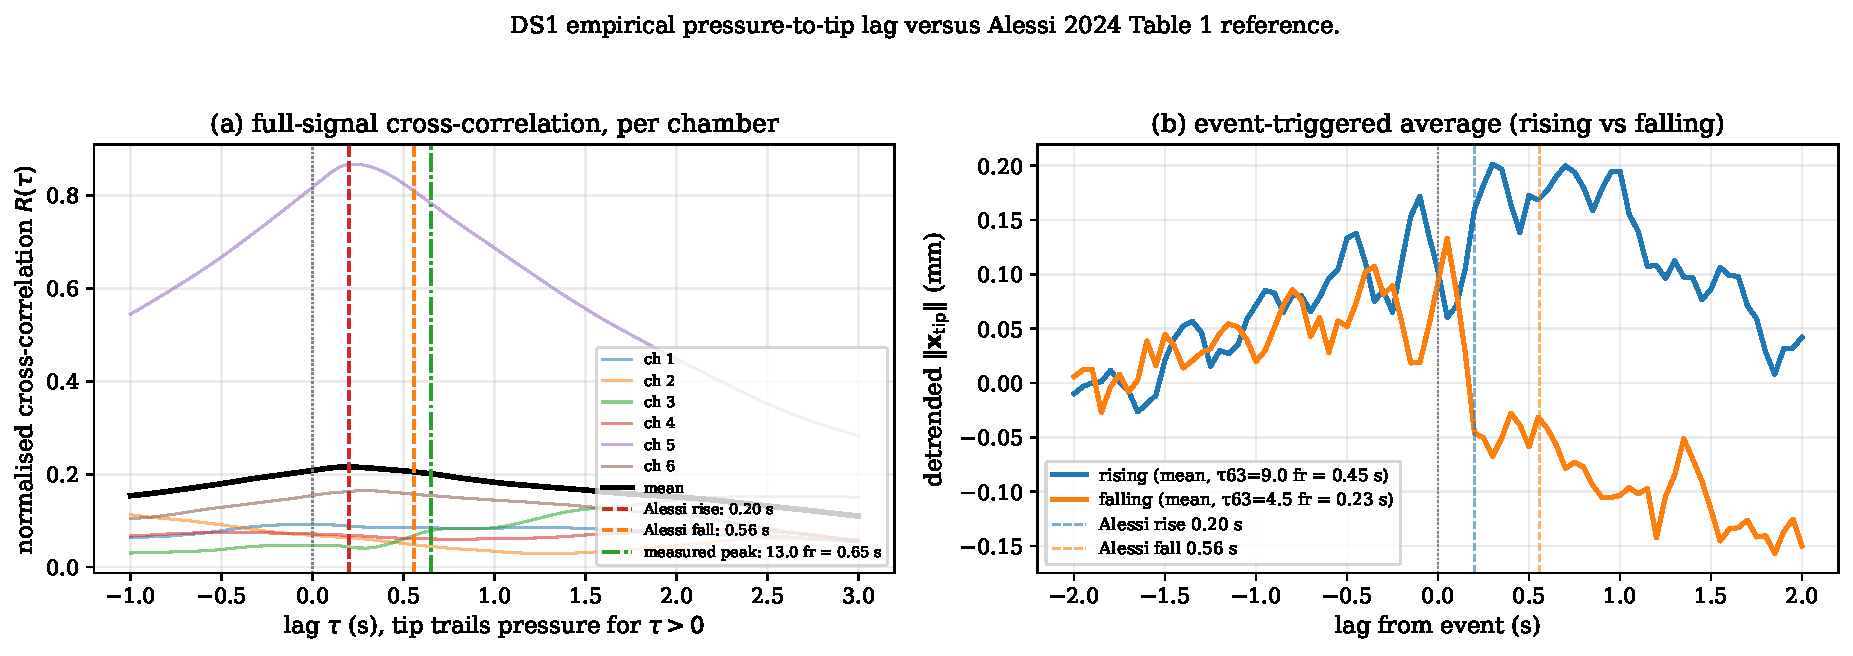
\includegraphics[width=0.98\linewidth]{fig/ds1_pressure_tip_lag.pdf}
  \caption[DS1 empirical pressure-to-tip lag against Alessi 2024.]{Empirical pressure-to-tip lag on Dataset~1's training frames (seeds~1 and 2, $N = 7981$) compared with Alessi et al.\ \cite{alessi2024pushing} Table~1. (a) Normalised cross-correlation $R(\tau)$ of each chamber's pressure against the tip-displacement magnitude; chamber~5 peaks at $\tau = 5$ frames ($0.25$\,s) with $R = 0.87$, within one frame of the $0.2$\,s pressurisation time. The median absolute peak lag across all six chambers is $13$ frames. (b) Event-triggered average of the tip-displacement response to dp/dt extrema (rising and falling templates, mean over six chambers); the random-walk excitation does not cleanly isolate Alessi's asymmetric load/unload transients, but the order-of-magnitude lag agreement is sufficient to motivate a recurrent window $K \geq 10$ frames.}
  \label{fig:app_ds1_lag}
\end{figure}

\section{Reproducibility}
\label{app:reproducibility}

Table~\ref{tab:app_repro_env} lists the software and hardware environment in which every experiment of Chapter~\ref{chap:results} was executed. All numbers reported in this thesis were generated on this single workstation with a fixed random seed of $42$ and cuDNN set to deterministic (\texttt{deterministic=True}, \texttt{benchmark=False}); re-running the training scripts in the same environment reproduces the tabulated metrics to within the last displayed digit.

\begin{table}[!htbp]
  \centering
  \small
  \caption{Software and hardware environment used for all experiments.}
  \label{tab:app_repro_env}
  \begin{tabularx}{\linewidth}{@{}l X@{}}
    \toprule
    Component & Value \\
    \midrule
    Operating system        & Ubuntu 24.04.4 LTS (Linux 6.17.0) \\
    CPU                     & Intel Core i7-13650HX (14 cores, 20 threads) \\
    RAM                     & 16\,GB DDR5 \\
    GPU                     & NVIDIA GeForce RTX 4060 Laptop (8\,GB, CUDA 12.6) \\
    Python                  & 3.11 \\
    PyTorch                 & 2.11.0+cu126 \\
    torchvision             & 0.26.0+cu126 \\
    NumPy / Pandas / SciPy  & 2.4.3 / 3.0.2 / 1.17.1 \\
    scikit-learn            & 1.8.0 \\
    matplotlib              & 3.10.8 \\
    PyElastica              & 0.3.3.post2 \\
    Random seed             & $42$ (Python, NumPy, PyTorch CPU and CUDA) \\
    cuDNN flags             & \texttt{deterministic=True}, \texttt{benchmark=False} \\
    Outer repository commit & \texttt{e9a7d5d} (\textit{soft\_robot\_ai}) \\
    \bottomrule
  \end{tabularx}
\end{table}

\paragraph{Checkpoint layout.}
All trained networks are stored under \texttt{checkpoints/\{experiment\}/\{run\_id\}/best.pt}, where \texttt{experiment} is one of \{\texttt{mlp\_ds1\_tip}, \texttt{mlp\_ds1\_tipmid}, \texttt{mlp\_ds2\_tip}, \texttt{lstm\_ds1\_tip}, \texttt{lstm\_ds1\_tipmid}, \texttt{lstm\_ds2\_tip}, \texttt{fk\_ds1}, \texttt{fk\_ds2}, \texttt{sim2real\_A}, \texttt{sim2real\_B}, \texttt{sim2real\_C}\} and \texttt{run\_id} encodes the date and the configuration hash. Each checkpoint file is a single PyTorch dictionary with keys \texttt{model\_state\_dict}, \texttt{optimizer\_state\_dict}, \texttt{config} (the full YAML used for training), \texttt{input\_scaler}, \texttt{output\_scaler}, \texttt{seed}, \texttt{git\_hash}, and \texttt{timestamp}, following the metadata convention of Section~\ref{sec:reproducibility}.

\paragraph{Evaluation determinism.}
Evaluation scripts load the checkpoint, restore both scalers, re-seed all random-number generators, and run a single forward pass over the frozen test split. No test-time augmentation, dropout, or batch-normalisation update is applied. Closed-loop tracking evaluations use the fixed reference trajectories of Section~\ref{sec:traj} and the same FK arbiter checkpoint for every method, so that any differences between methods are attributable to the methods themselves rather than to arbiter variation.

\paragraph{Code availability.}
The training scripts, evaluation pipelines, configuration files, and figure-regeneration scripts are archived in the project repository described in Appendix~\ref{app:code}. The exact commit associated with the numbers reported in Chapter~\ref{chap:results} is \texttt{e9a7d5d} on the \texttt{master} branch; the raw Dataset~1 pickles and the Dataset~2 CSV are held under \texttt{data/raw/} and are not redistributed because of upstream licensing constraints stated in Appendix~\ref{app:code}.

\chapter{Code Availability}
\label{app:code}

% TODO: link to the code repository.
Codes are available at: \url{https://github.com/zhongm-525/Dissertation.git}


\end{document}
